\chapter{Расчетные исследования известных схем}\label{ch:ch2}

Начнем с очерчивания рамок расчетного исследования.
Оставляя в стороне вопросы, связанные с химической переработкой для получения восстановленной урановой изотопной смеси, предлагается рассмотрение усовершенствованных каскадов газовых центрифуг для повторного обогащения этой смеси для производства низкообогащенного урана. 

В расчетных задачах ограничимся следующими предположениями:

 \begin{enumerate}
  \item регенерированный ураном, получен из ОЯТ легководного энергетического реактора. В качестве примера будем рассматривать изотопный состав регенерата из реактора российского дизайна -- ВВЭР.
  \item коэффициент разделения характерен центрифуге российского дизайна.
\end{enumerate}

\section{Обоснование ограничений использования ординарных схем (на основе ординарных каскадов)}\label{sec:ch2/sec1}


Таким образом, анализ схем на основе базового трехпоточного каскада демонстрирует потребность в модификации компоновок разделительного оборудования в контексте многократного рецикла урана.

Подводя итог подраздела, известные на сегодняшний день  технические решения основаны на:
-	разбавлении регенерированного урана материалами, не содержащими минорных компонентов (например, природным ураном), на входе в разделительный каскад, на выходе из разделительного каскада или внутри каскада при наличии в нем двух питающих потоков (регенерат и разбавитель);
-	получении регенерата с пониженным содержанием минорных изотопов в каскаде с двумя питаниями и двумя потоками продукта (отбора);
-	выделении из смесей регенерированного урана изотопа $^{232}$U при помощи газа-носителя в последовательном соединении двух разделительных каскадов.

\section{Обоснование необходимости составных схем/схем с дополнительными потоками}\label{sec:ch2/sec2}
Из вышепреведенного обоснования невозможности решения задачи полного возврата регенерата в топливный цикл легководных реакторов в условиях многократного рецикла и вытекает необходимость использовать составные каскадные схемы ввиду необходимости  `пространственного' разделения. Так двойная схема позволяет отделить минорные легкие изотопы $^{232}$U, $^{234}$U в независимом потоке отборной части каскада. Так, например, схема \ref{fig:double} позволяет во втором каскаде разделить потоки, выделив $^{235}$U в тяжелой фракции, направив $^{232}$U и $^{234}$U в легкую.

\begin{figure}[ht]
  \centerfloat{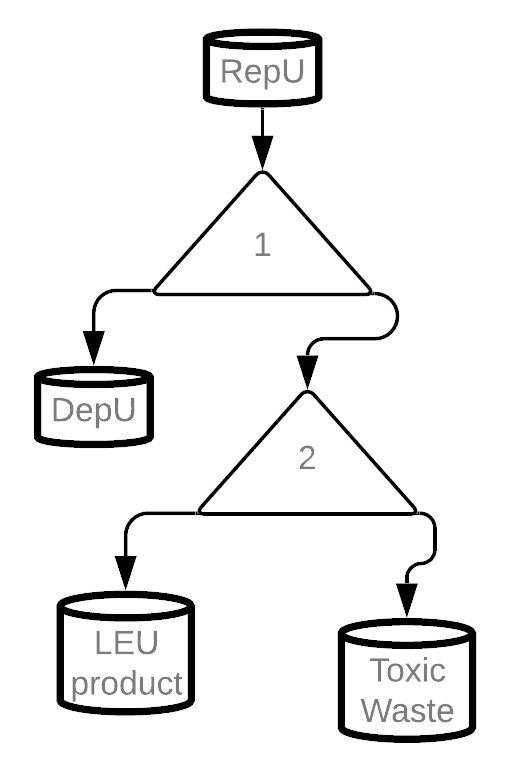
\includegraphics[scale=0.3]{cascades/double}}
  \caption{Двойной каскад}\label{fig:double}
\end{figure}

С появлением свойств такого рода у каскадов, вместо привычной дихотомии, выделяющей схемы с приставкой `много-' (многопоточные схемы, многокаскадные конфигурации), предлагается классифицировать каскады, используемые для обогащения регенерата, как разбавляющие или очищающие. Так, схема двойного каскада является очищающей, в отличие от схем, основанных на ординарном каскаде, работающих на принципе разбавления.  Хоть и любая таксономия арбитрарна (\textcolor{red}{позиция номиналистов в споре с реалистами}
), условная граница `каскад-разбавитель' -- `каскад-очиститель' гораздо лучше подчеркивает сущностные характеристики анализируемых схем, предназначенных для повторного обогащения урана.
 

\section{Разработка схем полного возврата}\label{sec:ch2/sec3}
\subsection{Модифицированный двойной каскад}

В качестве модификации двойного каскада была предложена альтернативная каскадная схема, которая позволяет обеспечить возврат регенерата в цикл в соотношении 1:1. В этой схеме, изображенной 
на рисунке \ref{fig:vestnik}, первая часть (каскад 1) увеличивает 
концентрацию $^{235}$U со всеми более легкими изотопами ($^{232}$U и $^{234}$U) и направляет их (через выходящий поток в правой части на рисунке) ко второму каскаду, который будет концентрировать эти четные миноры в потоке загрязненного продукта \cite{smirnovObogashchenieRegenerirovannogoUrana2018}.
Хотя на этот раз приготовленная композиция разбавляется НОУ для контроля концентраций $^{232}$U и $^{234}$U в допустимых пределах и для управления соотношением рециклируемых материалов (для поддержания соотношения регенерата в питании каскада к нарабатываемому продукту на уровне 1:1, что формально соответствует полному возврату выгоревшего топлива в ядерный топливный цикл).

\begin{figure}[ht]
  \centerfloat{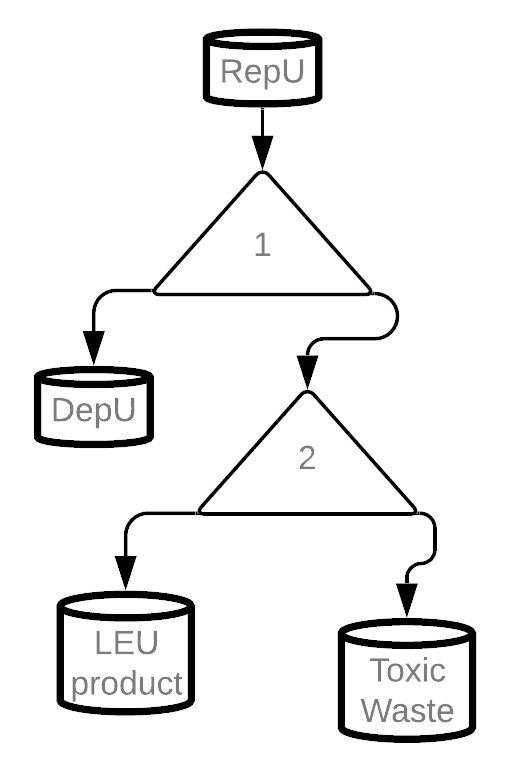
\includegraphics[scale=0.3]{cascades/double}}
  \caption{Двойной каскад с добавлением НОУ (тройной каскад)}\label{fig:vestnik}
\end{figure}

Хотя этот вариант и кажется идеальным, цена хранения побочного продукта из загрязненной смеси слишком высока, что мгновенно делает схему нежизнеспособной, если нет способов избежать такого негативного побочного эффекта.
Однако затем было предложено применить дополнительный каскад для производства НОУ из загрязненной смеси, сильно разбавленной обедненным ураном (которые имеют высокую концентрацию $^{235}$U около $\approx$20\%), чтобы получить конечный продукт в двух исходящих потоках и достичь значительной экономии природного урана ($\approx$38\%) даже для `грязной' композиции, которая уже была пятикратно рециклирована (рисунок \ref{fig:Tomsk}). Расчеты показали, что такой подход позволяет производить НОУ коммерческого качества, расходуя определенное количество переработанного урана и отвечая стандартным спецификациям для  $^{232}$U (и условиям, установленным для других четных изотопов). В то же время, предлагаемая схема обеспечивает большую экономию природного урана, чем большинство схем обогащения переработанного урана. Это могло бы также обеспечить широкомасштабную «мобилизацию» обедненного урана.

\begin{figure}[ht]
  \centerfloat{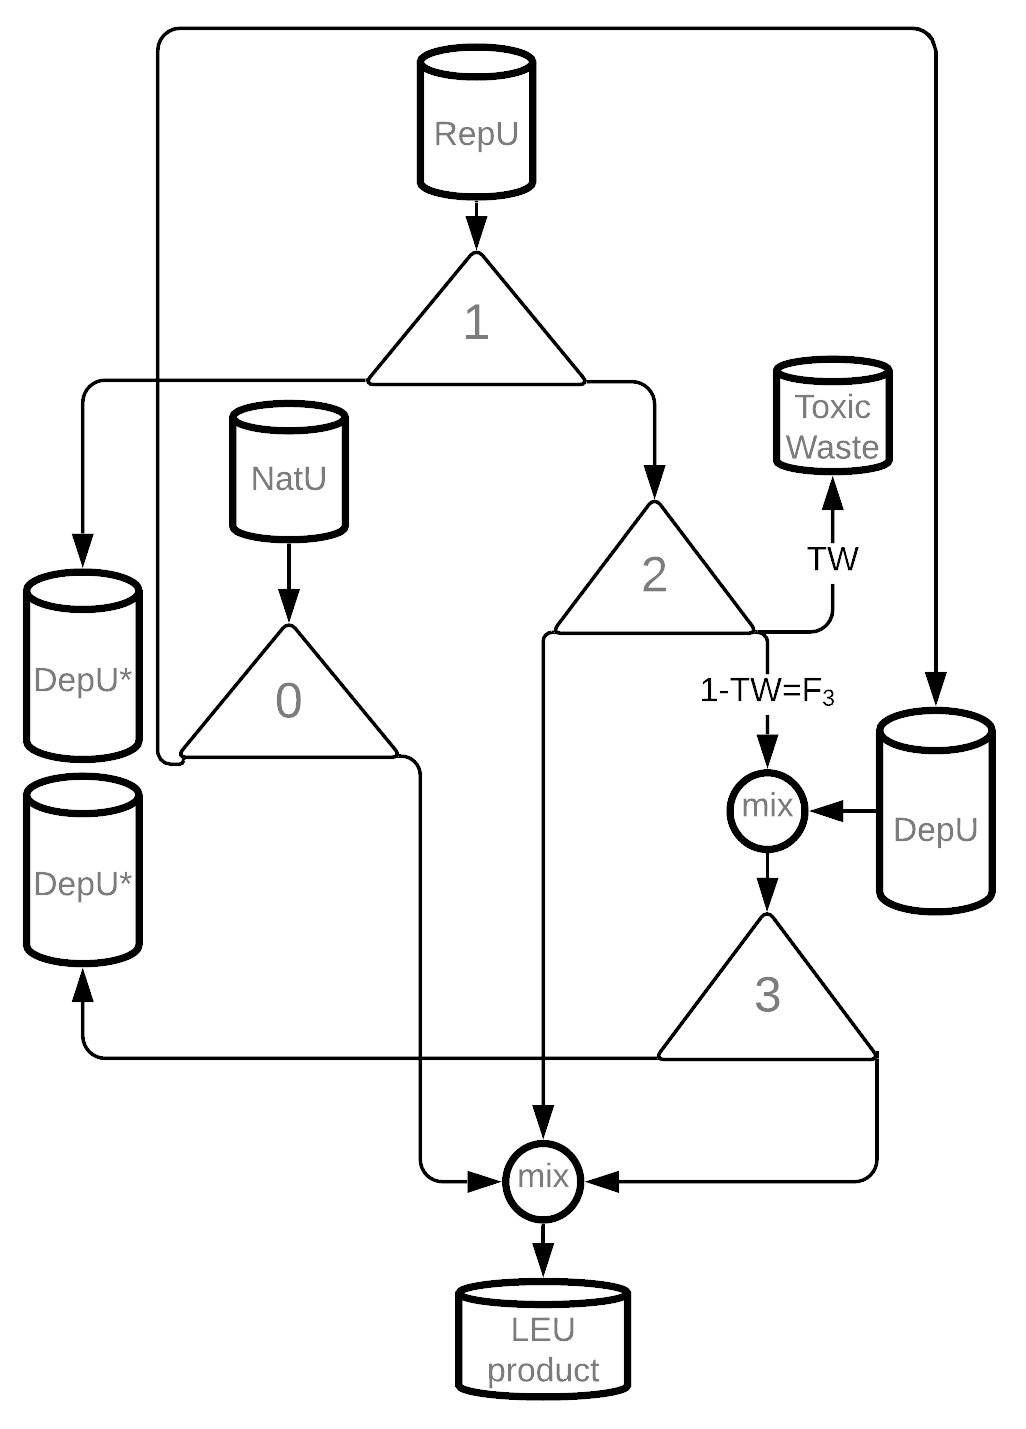
\includegraphics[scale=0.3]{cascades/Triple_Tomsk}}
  \caption{Тройной каскад с подмешиванием ОГФУ и НОУ-разбавителем}\label{fig:Tomsk}
\end{figure}

Затем, в качестве альтернативы была предложена схема рисунка \ref{fig:patent}), в которой на каскад с индексом 3 подается смесь грязного потока легкой фракции каскада 2, которая разбавляется обедненным гексафторидом урана до содержания $^{235}$U на уровне природного урана. Этот поток в дальнейшем разбавляется чистым природным ураном, пропорция которого подбирается для выполнения всех заданных условий.
\begin{figure}[ht]
  \centerfloat{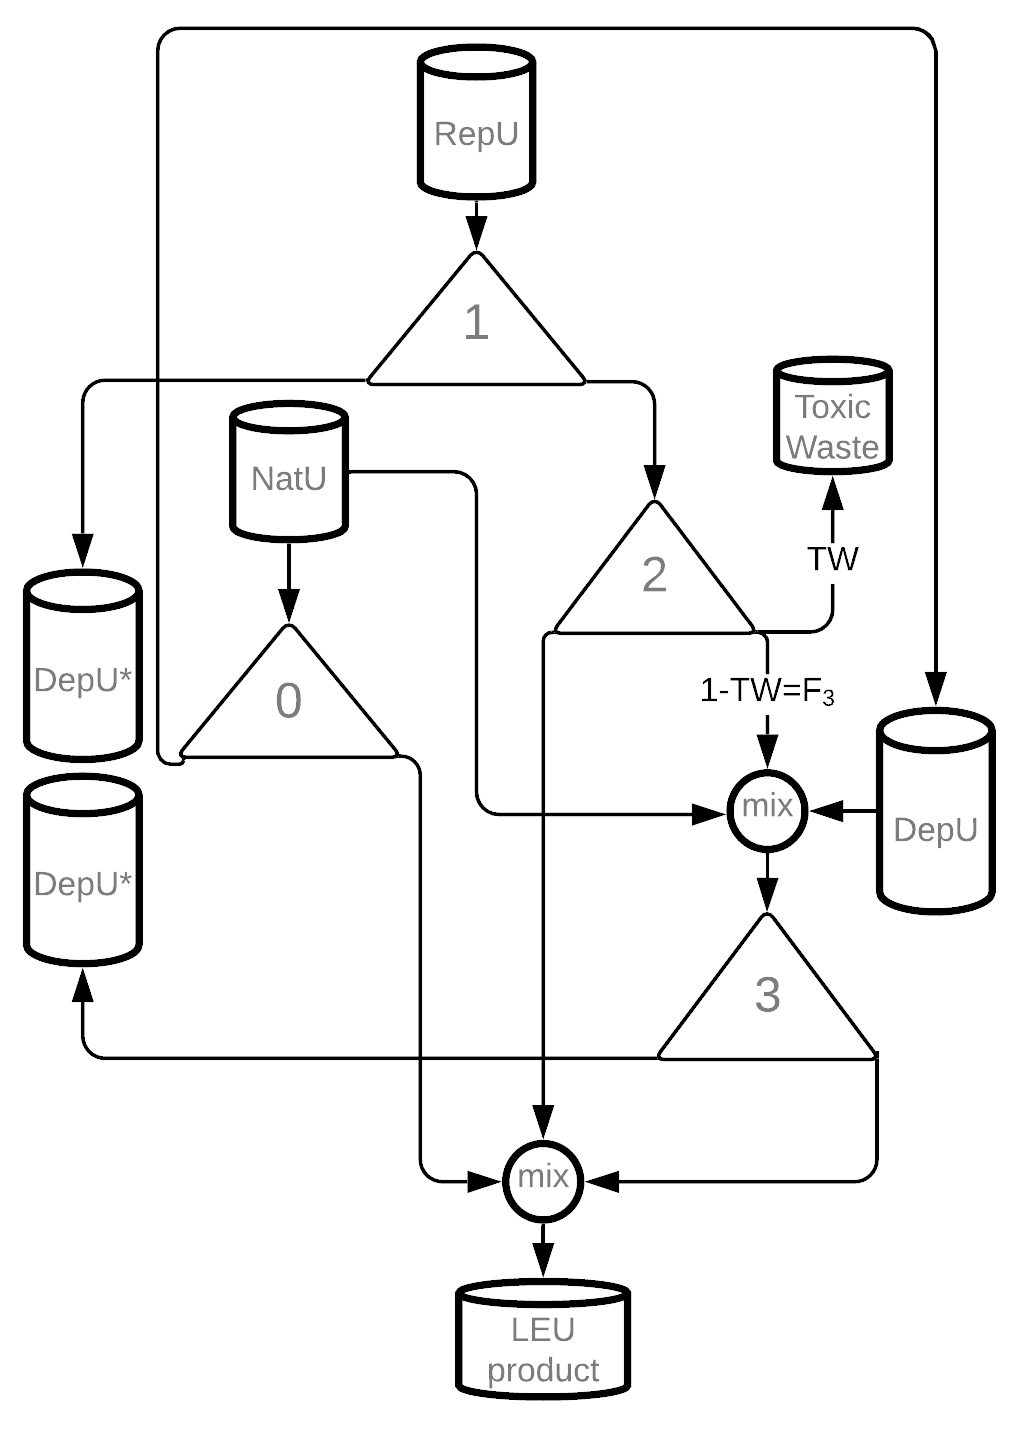
\includegraphics[scale=0.3]{cascades/triple_cascade_complete_return}}
  \caption{Тройной каскад с подмешиванием НОУ, ОГФУ и природного урана}\label{fig:patent}
\end{figure}

Как мы видим, такие схемы также очень ценны как инструмент для переработки предписанного количества выделенного урана.

Хранение загрязненного побочного продукта сопряжено с существенными дополнительными затратами, поэтому важен поиск способов избежать накопления этого материала.
Исходя из этого, в работе \cite{smirnovMethodEnrichReprocessed2019} предложено применить дополнительный каскад.
Далее будет предложен краткий обзор такого каскада.

\subsubsection{Анализ влияния ограничений предельно допустимой концентрации $^{232}$U в товарном НОУ}

Анализ результатов таблиц  показывает, что рассматриваемая модификация двойного каскада позволяет многократно обогатить рециклированный уран при различных внешних ограничениях, касающихся концентрации $^{232}$ в продукте и величины потока возвращаемого в воспроизводство топлива регенерированного урана. При этом уменьшение допустимой кон-центрации $^{232}$ в продукте при фиксированном отношении (исходный регенерат)/(товарный НОУ) обусловливает существенное снижение экономии природного урана и изменение числа центрифуг в каскадной схеме. Например, при отношении регенерата к конечному продукту на уровне 0,93 экономия природного урана уменьшилась, а перерасход работы разделения увеличился примерно в 2 раза при изменении ограничения на $^{232}$ от 5·10-7 до 1·10-7. Однако введение более жёстких ограничений на 232U способствовало одновременному снижению концентрации и остальных чётных изо-топов в получаемом продукте, особенно $^{236}$. Данный фактор является положительным в случае многократного рециклирования урана, по-скольку будет обеспечивать меньшее содержание $^{232}$ на последующих рециклах [30].
В дальнейшем отдельного изучения требует вопрос оптимального выбора концентрации в потоке P2 второго каскада. В рамках настоящей работы рассматривали случай, когда данная концентрация не превышала 20\%, что соответствует порогу, принятому МАГАТЭ для материала прямого использования [31]. Однако в некоторых работах, в которых рассматривают двойные каскады для обогащения регенерата, указанная концентрация заметно (в 2 раза и более) превышает величину 20\%. Увеличение данной концентрации, очевидно, может уменьшить количество получаемого радиоактивного отхода, а также обеспечить более эффективное удаление $^{232}$ из продукта.


\subsection{Четверной каскад}

Схема каскада, состоящего из четырех ординарных каскадов решает проблему обращения с легкой фракцией, вышедшей из второго каскада.
Это позволяет вовлечь больше $^{235}$U, и избавляет от необходимости конечной утилизации материала с высоким содержанием $^{232}$U.
Принцип работы такой схемы состоит в следующем.
Теперь финальный продукт -- низкообогащенный уран -- получается путем смешения двух потоков.
Первый из них аналогичен финальному продукту, полученному посредством тройной схемы рис. \ref{fig:triple}.
Второй же нарабатывается из загрязненной смеси, сильно разбавленной обедненным ураном.
При этом, конфигурация подбирается таким образом, чтобы на получение единицы продукта из этих совмещенных потоков затрачивалось требуемое количество ($\approx$0.93) питающего регенерата.

Итак, данная схема позволяет получить конечный продукт в двух исходящих потоках и достичь значительной экономии природного урана (~ 38\%) даже для «грязного» регенерата, которая уже была пятикратно переработана.
При этом, для того же исходного состава регенерата, тройная схема показывает лишь (~ 8\%) в сокращении расхода природного урана в сравнении с ординарным, обогащающим природный уран \cite{smirnovObogashchenieRegenerirovannogoUrana2018}.
Однако такой эффект связан с двухкратной работой разделения, требуемой четверной схеме, тогда как тройная схема затрачивает лишь (~ 13\%) дополнительных РР.
Это связано с большим объемом вовлечения ОГФУ для разбавления загрязненного потока легкой фракции второго каскада.
Расчеты показали, что такой подход позволяет производить НОУ коммерческого качества, расходуя должное количество переработанного урана, в то же время отвечая стандартным спецификациям $^{232}$U (и условиям, установленным для других четных изотопов).
В то же время, предлагаемая схема обеспечивает более существенную экономию природного урана, чем большинство схем обогащения регенерированного урана.
Такая схема позволяет также обеспечить широкомасштабную «мобилизацию» обедненного урана.

\section{Сравнение схем полного возврата}

В данной части проводится сравнительный анализ каскадов, предназначенных для возврата регенерированного урана в ЯТЦ.
Рассматривается случай, когда схема производит эквивалентное количество продукта НОУ, затраченному регенерату.
Чтобы моделировать многократную переработку ядерного топлива, в качестве сырья используется регенерат, прошедший пять последовательных циклов.
Ключевые характеристики, связанные с общей эффективностью, такие как экономия природного урана, расход работы разделения и энергозатраты, были оценены для каждой схемы в удельных единицах (на единицу продукции).
Затем они были нормированы на величины, характерные для ординарного каскада(трехпоточного).
Чтобы избежать стоимостных показателей затрат, была использована методология пересчета ключевых показателей (экономия природного урана, объем обогащаемого ОГФУ и затраты работы разделения) в единицы потребляемой энергии (мегаватт-часы)  \cite{rodionovaAnalizTehnikoekonomicheskihHarakteristik2019}.
Этот показатель был предложен в качестве универсального инструмента оценки рассматриваемых каскадов, используемых для повторного обогащения урана.


